\documentclass{article}
\usepackage[T1]{polski}
\usepackage[utf8]{inputenc}
\usepackage[margin=1in]{geometry}
\usepackage[table]{xcolor}% http://ctan.org/pkg/xcolor
\usepackage{graphicx}
\usepackage{amssymb}

\begin{document}

\begin{titlepage}
    \begin{center}
        \vspace*{1cm}
        
        \Huge{Sprawozdanie do Projektu końcowego}
        
        
        \vspace{1.5cm}
        
        \large \textbf{Arkadiusz Duliban} \\
        \large \textbf{Wiktor Gruszczyński}
        
        \vfill
        
        
        \vspace{0.8cm}
        

        
        Politechnika Śląska\\
        Wydział Matematyki Stosowanej\\
        Kierunek Informatyka\\
        Inżynierskie, stacjonarne, sem. VII\\
        Rok akademicki 2017/2018
\\
        Gliwice
        
    \end{center}
\end{titlepage}

\newpage

\tableofcontents

\newpage

\vspace*{1in}

\section{Temat projektu}
Tematem projektu jest zaimplementowanie i porównanie kilku przykładowych algorytmów służących do przeszukiwania grafów: przeszukiwanie wszerz (BFS), przeszukiwanie w głąb (DFS), General Best First (GBF) oraz A*. 
\section{Cel projektu}
Naszym celem jest zaimplementowanie algorytmów BFS, DFS, GBF oraz A*. W tym celu stworzone zostanie narzędzie służące do demonstracji działania algorytmów przeszukiwania grafów. Porównywanie będzie się odbywać poprzez znajdowanie drogi między dwoma punktami umieszczonych na planszy składającej się z siatki kwadratów o wymiarze n x n. Dodatkowo niektóre elementy siatki będą mogły zostać wyłączone – tzn. droga nie będzie mogła przeciąć żadnego z nich. 
Algorytmy zostaną przetestowane dla różnych wariantów danych wejściowych (położenia punktu startowego i końcowego,  inna konfiguracja i liczebność przeszkód). Porównane zostaną: liczba iteracji, długość drogi, ilość wyznaczonych sąsiadów.
\section{Sposób realizacji projektu}
Projekt zostanie przygotowany w formie aplikacji webowej. Użytkownik będzie zadawać parametry wejściowe poprzez modyfikowanie interaktywnego schematu mapy (w postaci siatki). W ten sposób będzie dokonywany wybór punktu startowego, końcowego oraz bloków – przeszkód. Algorytm będzie wywoływany po każdorazowej akcji wykonanej przez użytkownika. 
Do uruchomienia aplikacji wystarczy przeglądarka internetowa wspierająca obsługę elementu canvas (każda zaktualizowania na przełomie ostatnich 3-4 lat). Uruchomić należy plik \textbf{index.html }
\section{Komentarz do zadania} 
\begin{enumerate}
	\item Stworzono graf – „mapę” do przeszukiwania. Mapa składa się z n wierszy (rowsCount) oraz z m kolumn (boxPerRow). Mapa opisywana jest poprze tablicę net składającą się z n∙m obiektów, których struktura przedstawia się następująco: 
	\begin{itemize}

		\item x    - pozycja poziomo (w pikselach) obiektu na graficznych odwzorowaniu siatki
		\item y   - pozycja pionowo (w pikselach) obiektu na graficznych odwzorowaniu siatki
		\item type  - rodzaj bloku (startowy, końcowy, przeszkoda, zwykły)
		\item neighId – jeśli blok jest sąsiadem, zmienna przechowuje informacje, który z kolei jest to sąsiad
		\item isSearched – czy element był brany pod uwagę przy poszukiwaniach
		\item lastSearched – czy element występował jako ostatni przy przeszukiwaniu
	\end{itemize}
	Do prawidłowego działania algorytmu jest wymagana jedynie zmienna type.  Pozostałe są użyte jedynie w celu wizualizacji wyniku. 
	
	\newpage
	\item Zaimplementowane zostały kolejno wszystkie z algorytmów.
Procedury BFS{\_}search,  DFS{\_}search jako parametr początkowy przyjmują numer bloku startu oraz numer bloku końca. Procedura GBF{\_}search z kolei wymaga podania dokładnie tych samych parametrów oraz – dodatkowo – referencji do funkcji heurystycznej A lub B. Związane jest to z tym, iż algorytm pozwalamy uruchomić w dwóch konfiguracjach, z różnymi heurystykami. \\
Jako wynik otrzymywane są dwie listy:
	\begin{itemize}
		\item lista zawierająca kolejne numery bloków tworzących wyznaczoną trasę między blokami startu i końca (A i B)
		\item lista składająca się z list zawierających identyfikatory sąsiadów punktów wyznaczanych w kolejnych 
	\end{itemize}
	\item Wyniki algorytmów przedstawiane są na sąsiadujących ze sobą „mapach” – obiektach typu canvas. Każde kliknięcie (akcja) powoduje wywołanie funkcji uruchamiającej algorytm – OnCanvasClick(). Rolę pomocniczą pełni funkcja ChangeSquareType(), która zmienia typ ostatnio klikniętego obiektu: jeśli nie było jeszcze bloku startowego – w start; jeśli nie było końcowego – w końcowy; jeśli jest to blok zwykły – w przeszkodę; jeśli jest to blok inny niż zwykły – zamienia blok w blok zwykły. \\
Za rysowanie jest odpowiedzialna funkcja DrawNet, która rysuje siatkę na mapie zadanej jako argument. Wszelkie dane potrzebne do wyrysowywania obiektu pochodzą z danych wyjściowych algorytmu. 
	\item Dodatkowo skonstruowane narzędzie zostało wyposażone w następujące opcje:
	\begin{itemize}
			\item Możliwość wyświetlenia na mapie sytuacji aktualnej dla i-tej iteracji. W tym celu wywoływana jest funkcja SetIteration(i) – wyświetlanie wyniku jest ograniczone i nie wyświetlamy wszystkich danych N iteracji, lecz wyświetlanie kończymy na iteracji i.
   			\item Odtwarzanie animacji przedstawiającej poszukiwanie drogi – realizowane przez funkcję playIterations(), która samoczynnie przestawia numer iteracji od 1 aż do N.
			\item Czyszczenie siatki ze zmian wprowadzonych poprzez uruchomienie algorytmu – funkcja EraseCanvas(clearAlsoObjects) odpowiada za zerowanie ustawień do stanu początkowego. Jako parametr przyjmowana jest zmienna logiczna informująca, czy należy również wyczyścić bloki startowe, końcowe i przeszkody. 
			\item Zmiana rozmiaru siatki net
	\end{itemize}
	\item Powyżej ograniczono się jedynie do wymieniania najważniejszych funkcji – dużą część kodu odgrywają funkcje pomocnicze oraz odpowiadające za interakcję z użytkownikiem aplikacji. 
\end{enumerate}


\newpage

\section{Algorytmy}
\subsection{Breadth First Search}
Przeszukiwanie wszerz, algorytm który wyszukuje znajdujące się pola jak najbliższej pola startowego. Dzięki temu każde nowe dodane pole wie jaka jest najkrótsza droga by do niego dotrzeć. Dzieje się to jednak kosztem dużej ilości iteracji. Algorytm poszukuje na ślepo w swoim najbliższym sąsiedztwie.
\begin{enumerate}
\item Zainicjowanie pamięci: stos, odwiedzone
\item Dodanie punktu początkowego do listy odwiedzonych oraz do stosu
\item Póki stos nie jest pusty:
	\begin{itemize}
	\item pobieranie punktu ze stosu
	\item znajdowanie jego sąsiadów
	\item dla każdego z sąsiadów:
	\begin{itemize}
		\item jeżeli dany punkt nie znajduje się w liście odwiedzonych:
			\begin{itemize}
			\item jeżeli punkt jest końcem:
				\begin{itemize}
				\item zwracanie ścieżki
				\end{itemize}
			\item w przypadku gdy punkt nie jest na liście odwiedzonych:
				\begin{itemize}
				\item dodawanie sąsiada na koniec stosu
				\item dodawanie sąsiada do listy odwiedzonych				
				\end{itemize}
			\end{itemize}
		\end{itemize}		
	\end{itemize}
\end{enumerate}

\subsection{Depth First Search}
Przeszukiwanie wgłąb, algorytm który przeszukuje pola kierujące się w daną stronę, sprawdzając najmłodsze dodawane pola do listy. Skutkiem tego algorytm może łatwo ominąć punkt leżący niedaleko od niego i wykonać sporą ilość iteracji zanim na niego trafi.

\begin{enumerate}
\item Zainicjowanie pamięci: stos, odwiedzone
\item Dodanie punktu początkowego do listy odwiedzonych oraz do stosu
\item Póki stos nie jest pusty:
	\begin{itemize}
	\item pobieranie punktu ze stosu
	\item znajdowanie jego sąsiadów
	\item dla każdego z sąsiadów:
	\begin{itemize}
		\item jeżeli dany punkt nie znajduje się w liście odwiedzonych:
			\begin{itemize}
			\item jeżeli punkt jest końcem:
				\begin{itemize}
				\item zwracanie ścieżki
				\end{itemize}
			\item w przypadku gdy punkt nie jest na liście odwiedzonych:
				\begin{itemize}
				\item dodawanie sąsiada na początek stosu
				\item dodawanie sąsiada do listy odwiedzonych				
				\end{itemize}
			\end{itemize}
		\end{itemize}		
	\end{itemize}
\end{enumerate}
\newpage
\subsection{Greedy Best-First Search}
Przeszukiwanie chciwe, algorytm który wykorzystuje heurystykę do znalezienia najkrótszej drogi w celu przeszukiwania najbardziej obiecujących pól. Pola o największym priorytecie (w przypadku tej implementacji o najmniejszej wartości zmiennej \textit{priority}) są brane wcześniej pod uwagę niż pola o niższym priorytecie. Dzięki temu algorytm kieruje się w stronę celu póki nie napotka przeszkód.
\begin{enumerate}
\item Zainicjowanie pamięci: kolejka priorytetowa, odwiedzone
\item Dodanie punktu początkowego do listy odwiedzonych oraz do kolejki
\item Póki kolejka nie jest pusta:
	\begin{itemize}
	\item zdejmowanie punktu z kolejki z najlepszym priorytetem
	\item znajdowanie jego sąsiadów
	\item dla każdego z sąsiadów:
	\begin{itemize}
		\item jeżeli dany punkt nie znajduje się w liście odwiedzonych:
			\begin{itemize}
			\item jeżeli punkt jest końcem:
				\begin{itemize}
				\item zwracanie ścieżki
				\end{itemize}
			\item w przypadku gdy punkt nie jest na liście odwiedzonych:
				\begin{itemize}
				\item dodawanie sąsiada do kolejki, z priorytetem równym heurystyce dystansu do punktu docelowego
				\item dodawanie sąsiada do listy odwiedzonych				
				\end{itemize}
			\end{itemize}
		\end{itemize}		
	\end{itemize}
\end{enumerate}


\subsection{A*}
A gwiazdka, algorytm który jest połączeniem algorytmu Dijkstry i chciwego. Wykorzystuje on funkcję kosztu przypisywaną do każdego pola. Algorytm, podobnie jak \textbf{GBF}, kieruje się najkrótszą drogą w stronę celu. Jednak jeżeli trafi na przeszkodę i będzie zmuszony się wrócić będzie on dalej w stanie wyznaczyć najkrótszą możliwą trasę. Dzieje się tak dzięki temu, że przy każdym znajdywaniu sąsiadów algorytm jeżeli uzna, że istnieje krótsza droga dojścia do danego pola nadpisuje ją. Sprawia to iż algorytm staje się bardziej czasochłonny lecz zawsze znajduje najkrótszą ścieżkę.  
\begin{enumerate}
\item Zainicjowanie pamięci: kolejka, odwiedzone
\item Dodawanie punktu początkowego do listy odwiedzonych oraz do stosu
\item Póki kolejka nie jest pusta:
	\begin{itemize}
	\item pobieranie punkt z kolejki z najlepszym priorytetem
	\item nadanie punktowi parametru kosztu - 0
	\item znajdowanie jego sąsiadów
	\item dla każdego z sąsiadów:
	\begin{itemize}
		\item jeżeli dany punkt nie znajduje się w liście odwiedzonych:
			\begin{itemize}
			\item jeżeli punkt jest końcem:
				\begin{itemize}
				\item zwracanie ścieżki
				\end{itemize}
			\item policzenie wartości nowego kosztu = koszt punktu z którego przybył + heurystyka dystansu pomiędzy znalezionym sąsiadem a punktem z którego przyszedł
			\item w przypadku gdy punkt nie jest na liście odwiedzonych lub nowy koszt jest mniejszy od parametru kosztu tego punktu:
				\begin{itemize}
				\item przypisanie sąsiadowi nowego parametru kosztu
				\item dodawanie sąsiada do kolejki, z priorytetem równym jego kosztowi + heurystyce od tego punktu do punktu celu
				\item dodawanie sąsiada do listy odwiedzonych				
				\end{itemize}
			\end{itemize}
		\end{itemize}		
	\end{itemize}
\end{enumerate}

\subsection{Porównanie}

\begin{itemize}
\item \textbf{i} - ilość iteracji
\item \textbf{n} - ilość przeszukanych sąsiadów
\item \textbf{s} - długość drogi
\end{itemize}

\subsubsection{Przykład 1}
\begin{center}
\begin{tabular}{c c c c c}
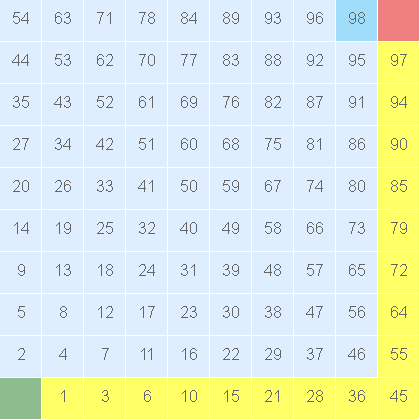
\includegraphics[scale=0.15]{images/scr.png} &
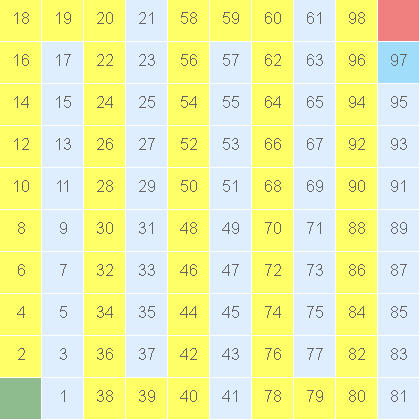
\includegraphics[scale=0.15]{images/scr1.png} &
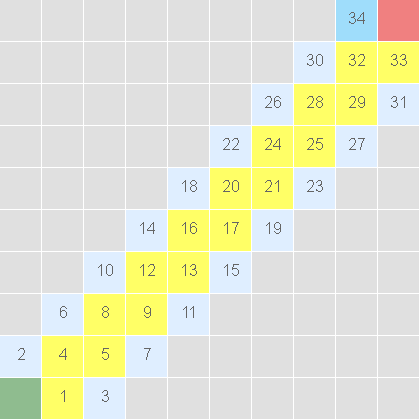
\includegraphics[scale=0.15]{images/scr2.png} &
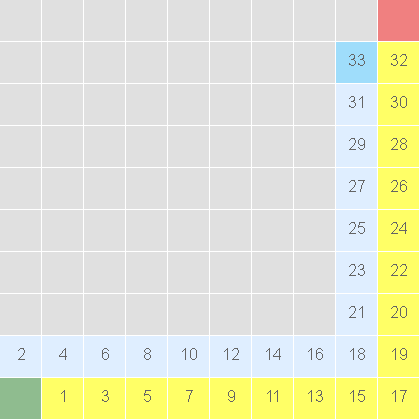
\includegraphics[scale=0.15]{images/scr3.png} &
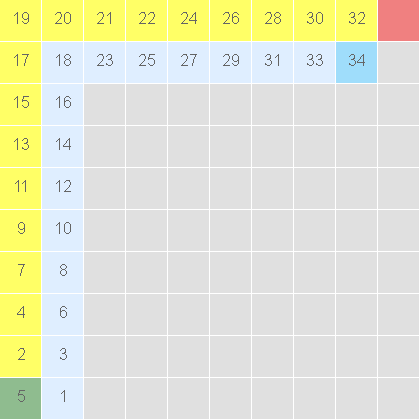
\includegraphics[scale=0.15]{images/scr4.png} \\
BFS & DFS & GBF A & GBF B & A* \\
i=89 & i=53 & i=17 & i=18 & i=18 \\
n=98 & n=98 & n=34 & n=33 & n=34 \\ 
s=19 & s=55 & s=19 & s=19 & s=19 \\
\end{tabular}
\end{center}
W tym przykładzie pokazana jest droga nie zakłócana żadnymi przeszkodami. Wszystkie algorytmy poza \textbf{DFS} były w stanie wyznaczyć najkrótszą ścieżkę. Algorytm \textbf{BFS} jednak musiał wykonać dużo iteracji i przeszukać wiele sąsiadów by błądząc trafić do pola końcowego. 

\subsubsection{Przykład 2}
\begin{center}
\begin{tabular}{c c c c c}
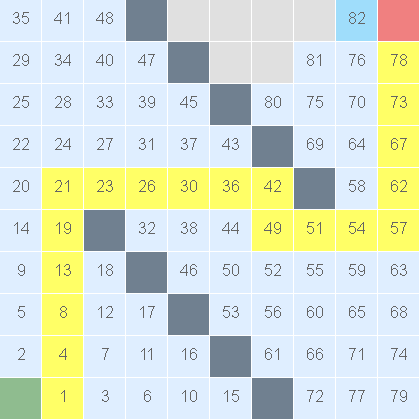
\includegraphics[scale=0.15]{images/scr5.png} &
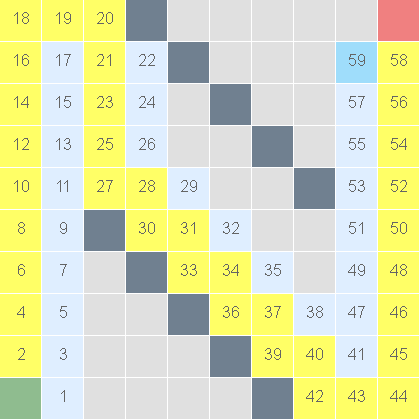
\includegraphics[scale=0.15]{images/scr6.png} &
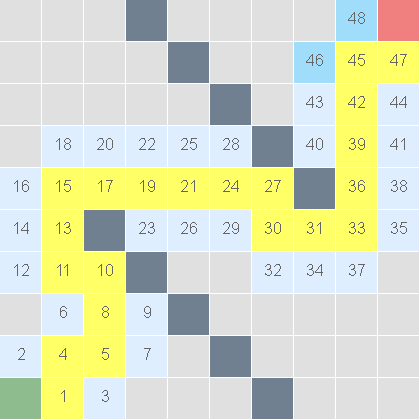
\includegraphics[scale=0.15]{images/scr7.png} &
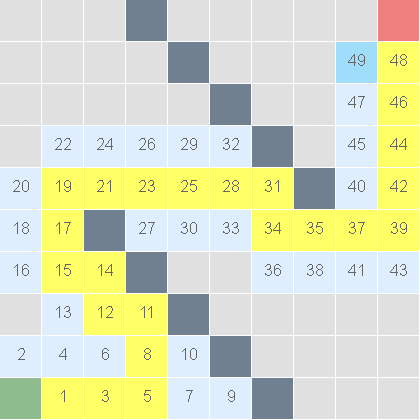
\includegraphics[scale=0.15]{images/scr8.png} &
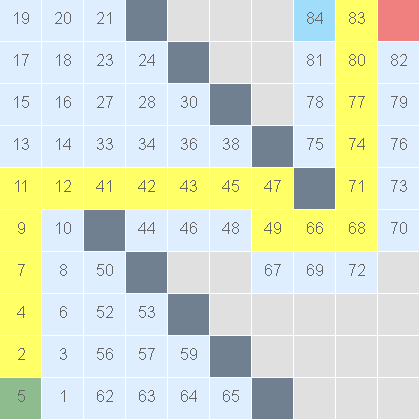
\includegraphics[scale=0.15]{images/scr9.png} \\
BFS & DFS & GBF A & GBF B & A* \\
i=64 & i=36 & i=21 & i=25 & i=51 \\
n=82 & n=59 & n=48 & n=49 & n=84\\
s=21 & s=37 & s=23 & s=25 & s=21\\
\end{tabular}
\end{center}
Ten przykład pokazuje jak potencjalnie zachowują się algorytmy napotykając przeszkodę w postaci ściany. Żadnemu z algorytmów nie zawsze znajdujących najkrótszą drogę (DFS, GBF) nie był w stanie wyznaczyć najkrótszej ścieżki. Algorytm \textbf{DFS} zgodnie ze swoim założeniem - sprawdza najmłodsze pola dodawane do stosu: najpierw pola w dół, następnie w górę, prawo i dopiero w lewo. Dlatego idąc w górę i ścieżka wyznaczona przez algorytm zatrzymuje się i skręca w prawo. Znowu napotykając przeszkodę, tym razem u dołu, postanawia pójść w prawo. Ale jak tylko jest możliwość znowu usiłuje iść w dół. Ten tok rozumowania sprawia, że ten algorytm poza kilkoma przypadkami nigdy nie znajdzie najkrótszej możliwej drogi. \\
Widoczny jest również problem algorytmów \textbf{GBF}, które mają problem gdy należy wrócić się z przeszukiwaniem. Szczególnie dobrze ilustrować będą to kolejne przykłady.\\

\subsubsection{Przykład 3}
\begin{center}
\begin{tabular}{c c c c c}
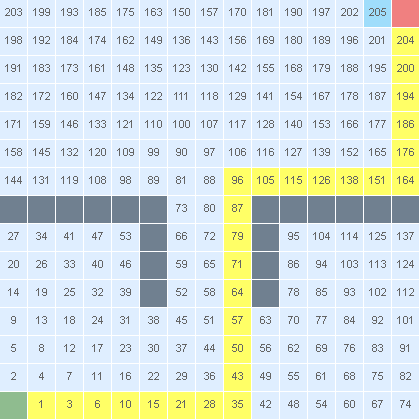
\includegraphics[scale=0.15]{images/scr10.png} &
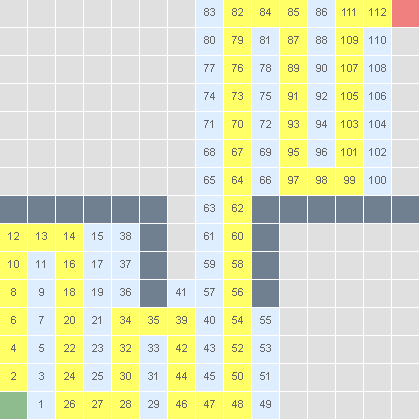
\includegraphics[scale=0.15]{images/scr11.png} &
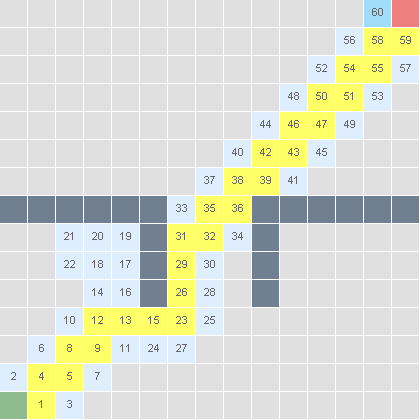
\includegraphics[scale=0.15]{images/scr12.png} &
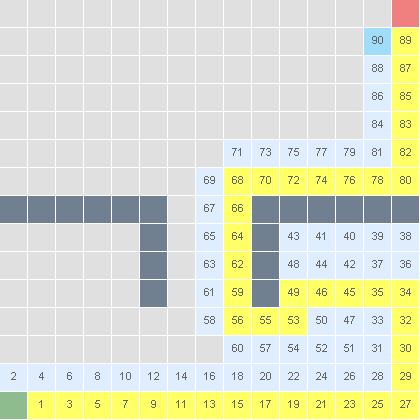
\includegraphics[scale=0.15]{images/scr13.png} &
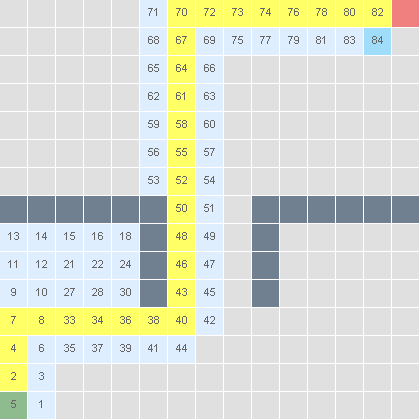
\includegraphics[scale=0.15]{images/scr14.png} \\
BFS & DFS & GBF A & GBF B & A* \\
i=179 & i=59 & i=32 & i=51 & i=43 \\
n=205 & n=112 & n=60 & n=90 & n=84\\
s=29 & s=59 & s=29 & s=43 & s=29\\
\end{tabular}
\end{center}
W tym przypadku jeszcze algorytmowi \textbf{GBF A} z heurystyką Euklidesa udaje się otrzymać ścieżkę z najkrótszą drogą przebytą. Dzieję się to dlatego iż przeszkody jedynie przecinają drogę do punktu końcowego wyznaczoną przez heurystykę algorytmu. Gorzej to wygląda w przypadku \textbf{GBF B}, gdzie użyty został dystans Manhattana. Ścieżka zwrócona przez algorytm musi się sporo wrócić.\\
Bardzo dobrze prezentuje się tu algorytm \textbf{A*}. Widać, że sprawdza on wszystkie pola we wgłębieniu a następnie efektownie wycofuje się z niego dając najkrótszą ścieżkę. 


\subsubsection{Przykład 4}
\begin{center}
\begin{tabular}{c c c c c}
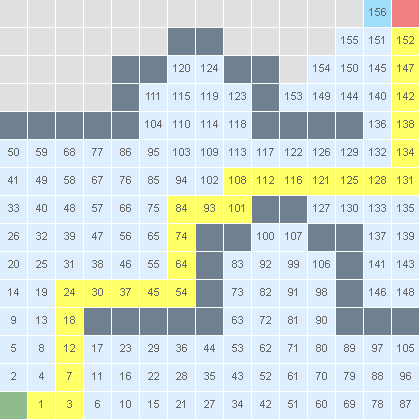
\includegraphics[scale=0.15]{images/scr25.png} &
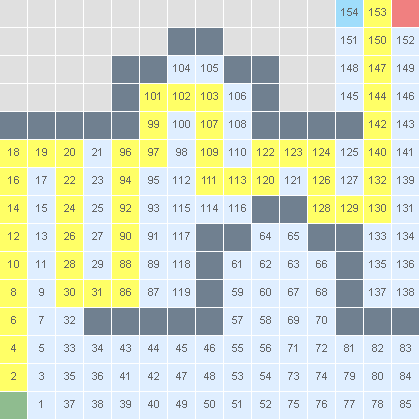
\includegraphics[scale=0.15]{images/scr26.png} &
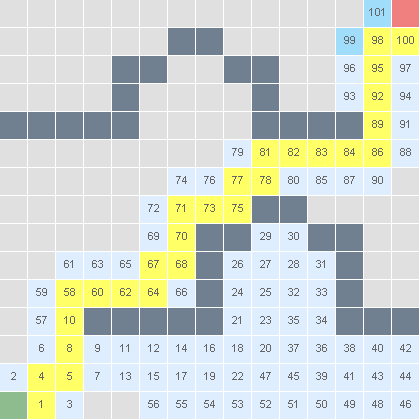
\includegraphics[scale=0.15]{images/scr27.png} &
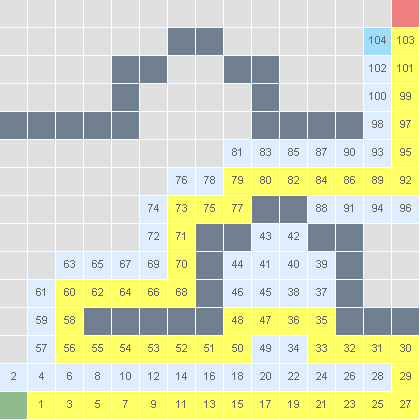
\includegraphics[scale=0.15]{images/scr28.png} &
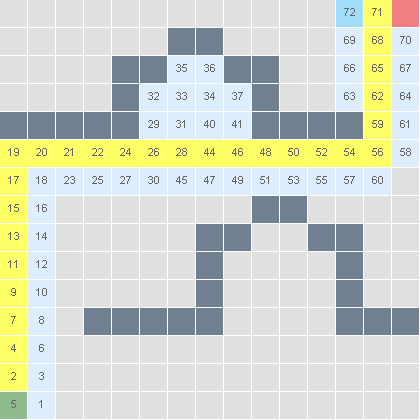
\includegraphics[scale=0.15]{images/scr29.png} \\
BFS & DFS & GBF A & GBF B & A* \\
i=123 & i=90 & i=60 & i=60 & i=37 \\
n=156 & n=154 & n=101 & n=104 & n=29\\
s=29 & s=49 & s=29 & s=55 & s=29\\
\end{tabular}
\end{center}
Implementacje \textbf{DFS} oraz \textbf{GBF B} znowu błądzą po mapie. Tutaj dobrze widać przewagę \textbf{A*} ponad pozostałymi algorytmami - nie robi on aż tyle zbędnych przeszukiwań i zawsze jest skuteczny.

\subsubsection{Przykład 5}
\begin{center}
\begin{tabular}{c c c c c}
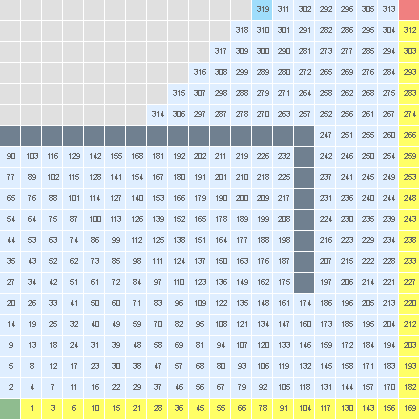
\includegraphics[scale=0.15]{images/scr31.png} &
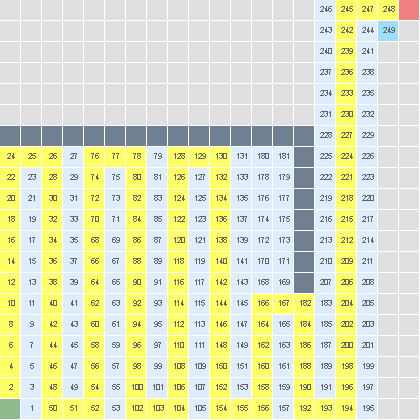
\includegraphics[scale=0.15]{images/scr32.png} &
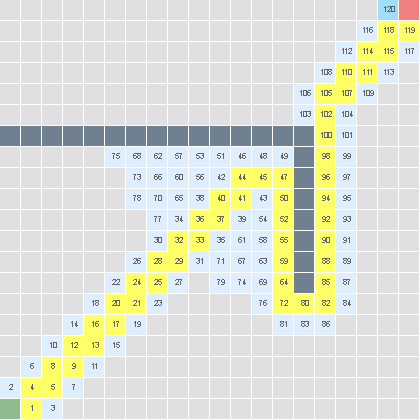
\includegraphics[scale=0.15]{images/scr33.png} &
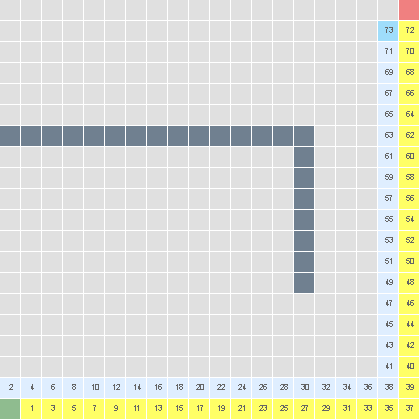
\includegraphics[scale=0.15]{images/scr34.png} &
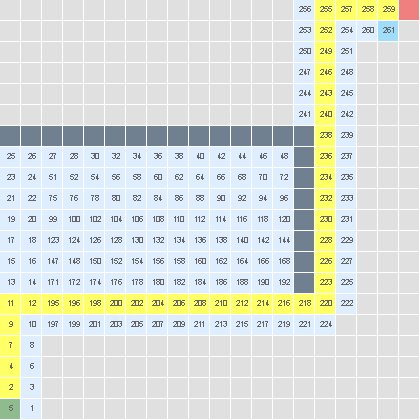
\includegraphics[scale=0.15]{images/scr35.png} \\
BFS & DFS & GBF A & GBF B & A* \\
i=292 & i=127 & i=74 & i=38 & i=136 \\
n=319 & n=149 & n=120 & n=73 & n=261\\
s=39 & s=121 & s=51 & s=39 & s=39\\
\end{tabular}
\end{center}
Znów widoczna jest wada algorytmów typu \textbf{GBF} - póki heurystyka nie napotka przeszkody takiej, która nie zmusza algorytmu do wracania z przeszukiwaniem algorytmy będą znajdować najkrótszą ścieżkę. \\ 
\textbf{A*} rozwiązuje ten problem robiąc porównania ścieżek prowadzących do danego pola od początku wielokrotnie, zawsze ustalając najkrótszą drogę dojścia do każdego pola.
\newpage
\subsubsection{Podsumowanie}

\begin{center}
\begin{tabular}{|c|c|c|c|c|}
\hline
& BFS & DFS & GBF & A* \\
\hline
zawsze najkrótsza możliwa ścieżka & \cellcolor{green} \checkmark & \cellcolor{red}X & \cellcolor{red}X &\cellcolor{green}\checkmark \\
\hline
\end{tabular}
\end{center}

Moim zdaniem najlepszym algorytmem jest \textbf{A*}. Znajduje on bowiem zawsze najkrótszą drogę, a to jest z reguły naszym zadaniem. Wykorzystuje on wskazywanie ogólnego kierunku drogi jak w przypadku \textbf{GBF} ale potrafi wyjść z "wklęsłości" bez stracenia na długości ścieżki. Algorytmy jak \textbf{DFS} oraz \textbf{GBF} nie dadzą najkrótszej ścieżki chyba, że będą mieć szczęście. \textbf{BFS} oraz A* to gwarantują, tylko \textbf{A*} robi to mniejszym kosztem (w większości przypadków).

\section{Implementacja}
Idea algorytmów jest prosta czego nie można powiedzieć o ich implementacji. W celu ułatwienia pracy stworzony został szereg pomocniczych funkcji i klas. 
\subsection{Elementy pomocnicze}
\subsubsection{Znajdowanie sąsiadów}
Funkcja odpowiedzialna za znajdowanie sąsiadów \textit{getNeighbours()} sprawdza czy na czterech polach można utworzyć ścieżkę. Robi to poprzez sprawdzenie czy pole: nad, po lewej, po prawej oraz pod zadanym w argumencie polem znajdują się w obrębie planszy oraz czy nie stoi na nich przeszkoda. Jako, że tablica w której przetrzymywane są dane na ten temat jest jednowymiarowa odbywa się to poprzez dzielenie modulo pozycji pola poprzez szerokość planszy.\\
Funkcja zwraca listę dostępnych pól.
\subsubsection{funkcja isOutOfRange()}
Funkcja sprawdza czy zadany identyfikator pola znajduje się na mapie.
\subsubsection{funkcja includesNode()}
Funkcja sprawdza czy w danej liście znajduje się obiekt typu \textit{node}.

\subsubsection{Klasa "node"}
Korzystając z dobrodziejstw języka \textit{JavaScript} utworzona została pomocnicza klasa \textit{node}, która miała oznaczać przeszukiwane pole. Podstawowymi atrybutami tej klasy są:
\begin{itemize}
\item \textbf{id} - oznaczające id danego pola w tablicy \textit{net}
\item \textbf{last} - będące odnośnikiem do \textit{node'a} z którego ten został wywołany
\end{itemize}\\
Klasa ta ułatwia odtwarzanie ścieżki utworzonej poprzez algorytmy.

\subsubsection{funkcja nodeToList()}
Funkcja ta odpowiedzialna jest za stworzenie listy identyfikatorów pól z listy obiektów typu \textit{node}. W argumencie podawany jest \textit{node}, z którego pobierany jest \textit{id} parametru \textit{last} i dodawany do listy zwrotnej. To samo dzieje się dla obiektu last i tak do końca. \\
W efekcie funkcja zwraca listę identyfikatorów ścieżki utworzonej z poprzedników \textit{node'a} podanego w argumencie.

\subsubsection{Kolejka priorytetowa}
Nasza implementacja nie jest do końca kolejką priorytetową tylko ją symuluje. \\
\begin{enumerate}
\item Tworzona jest lista \textbf{L}
\item Pętla:
	\begin{itemize}
	\item \textbf{L} jest odwracane
	\item \textbf{L} jest sortowane po priorytecie
	\item Operacje:
		\begin{itemize}
		\item ...
		\item dodaj element do \textbf{L} z danym priorytetem
		\item ...
		\end{itemize}				
	\end{itemize}
\end{enumerate}
\\
Lista jest odwracana by obiekty z najniższą liczbą priorytetową, czyli największym priorytecie, zawsze są brane pod uwagę wcześniej. \\
Początkowy algorytm działał źle gdyż nie brał on pod uwagi wieku dodanych elementów.
Dlatego wymyśliłem sztuczne obejście, które dodaje wiek elementom:
\begin{enumerate}
\item Tworzona jest lista \textbf{L}
\item \underline{Inicjuj iterator}
\item Pętla:
	\begin{itemize}
	\item \textbf{L} jest odwracane
	\item \textbf{L} jest sortowane po priorytecie
	\item Operacje:
		\begin{itemize}
		\item \underline{iterator++}
		\item ...
		\item dodaj element do \textbf{L} z danym priorytetem \underline{+ iterator*0.001}
		\item ...
		\end{itemize}				
	\end{itemize}
\end{enumerate}%

\subsection{Algorytmy}
Wszystkie algorytmy mają wspólne cechy:
\begin{enumerate}
	\item każdy algorytm zwraca:
	\begin{itemize}
		\item ścieżkę od początku do końca (jeżeli istnieje)
		\item historię przeszukiwanych pól
	\end{itemize}
	\item w argumentach wszystkich funkcji algorytmów podany jest początek i koniec, a w przypadku algorytmu \textbf{GBF} jeszcze typ heurystyki.
	\item ścieżka jest tworzona poprzez dodawanie do danego node'a parametru last, który ustanawia z którego pola można dojść do niego
	\item każde odwiedzone pole jest dodawane do historii przeszukiwanych pól
\end{enumerate}

\subsection{Heurystyki}
\begin{itemize}
\item Heurystyka A - dystans Manhattana\\
\begin{center}
$|bx-ax|+|by-ay|$
\end{center}
\item Heurystyka B - dystans Euklidesa\\
\begin{center}
$(bx-ax)^2+(by-ay)^2$
\end{center}
\end{itemize}

\end{document}

